\documentclass[english]{SPFShortReport}
\usepackage{subfigure}
\usepackage{spfFigures}
\usepackage{longtable}
\usepackage{url}
\usepackage{gensymb}
\usepackage[yyyymmdd,hhmmss]{datetime}
\reportName{Python calculation for heat pump SIN-22TU}
\reportSubName{Parametric Heat Pump calculation} 
\reportDate{\today \hspace{0.1cm} at: \currenttime \hspace{0.1cm} h} 
\author{Dani Carbonell}
\address{dani.carbonell@solarenergy.ch}
\begin{document}
\begin{table}[!ht]
\begin{small}
\caption{Fitted coefficients for the heat pump.}
\begin{center}
\resizebox{12cm}{!} 
{
\begin{tabular}{l | c c } 
\hline
\hline
Coefficient &Description & \\ 
 & &$[kW]$\\ 
\hline
$PQ_{1}$ & \emph{$1^{st}$ condenser polynomial coefficient}  & 2.2267e+01    \\ 
$PQ_{2}$ & \emph{$2^{st}$ condenser polynomial coefficient}  & 2.0015e+02    \\ 
$PQ_{3}$ & \emph{$3^{st}$ condenser polynomial coefficient}  & 4.1062e+01    \\ 
$PQ_{4}$ & \emph{$4^{st}$ condenser polynomial coefficient}  & -2.4655e+02    \\ 
$PQ_{5}$ & \emph{$5^{st}$ condenser polynomial coefficient}  & -2.0174e+02    \\ 
$PQ_{6}$ & \emph{$6^{st}$ condenser polynomial coefficient}  & -2.1232e+02    \\ 
\hline
$PCOP_{1}$ & \emph{$1^{st}$ COP polynomial coefficient}  & 5.6654e+00    \\ 
$PCOP_{2}$ & \emph{$2^{st}$ COP polynomial coefficient}  & 3.5744e+01    \\ 
$PCOP_{3}$ & \emph{$3^{st}$ COP polynomial coefficient}  & 3.3127e+00    \\ 
$PCOP_{4}$ & \emph{$4^{st}$ COP polynomial coefficient}  & -7.4772e+01    \\ 
$PCOP_{5}$ & \emph{$5^{st}$ COP polynomial coefficient}  & -1.5825e+02    \\ 
$PCOP_{6}$ & \emph{$6^{st}$ COP polynomial coefficient}  & -8.9463e+01    \\ 
\hline
$\dot m_{cond}$ & 4000.00 $[kg/h]$\\ 
$\dot m_{evap}$ & 4000.00 $[kg/h]$\\ 
\hline
$COP_{nom}$ (B0W35)& 4.57 \\ 
$Q_{c,nom}$ (B0W35)& 22.82 kW\\ 
$COP_{nom}$ (B2W35)& 4.77 \\ 
$Q_{c,nom}$ (B2W35)& 24.00 kW\\ 
$COP_{nom}$ (B10W35)& 5.44 \\ 
$Q_{c,nom}$ (B10W35)& 28.57 kW\\ 
\hline
\hline
\end{tabular}
}
\label{CoefTable}
\end{center}
\end{small}
\end{table}
\begin{table}[!ht]
\begin{small}
\caption{Predicting results of the heat pump.}
\begin{center}
\resizebox{12cm}{!} 
{
\begin{tabular}{l | c c c c c c c c c c c } 
\hline
\hline
$T_{evap,in}$ &$T_{evap,out}$ &$T_{cond,in}$ &$T_{cond,out}$ &$COP$ &$Q_{cond}$ &$Q_{evap}$ &$W_{comp}$ &$\dot m_{cond}$ &$\dot m_{evap}$ &$\Delta T_{evap}$ &$\Delta T_{cond}$ \\ 
$^oC$ &$^oC$ &$^oC$ &$^oC$ &$[-]$ &$[kW]$ &$[kW]$ &$[kW]$ &kg/h &kg/h &K &K\\ 
\hline
-7.00 & -10.28 & 26.02 & 30.00 & 4.02 & 18.51 & 13.90 & 4.61 & 4000 & 4000 & 3.3 & 4.0\\ 
-7.00 & -10.13 & 34.77 & 38.75 & 3.53 & 18.51 & 13.27 & 5.24 & 4000 & 4000 & 3.1 & 4.0\\ 
-7.00 & -9.78 & 43.61 & 47.50 & 2.87 & 18.13 & 11.80 & 6.33 & 4000 & 4000 & 2.8 & 3.9\\ 
-7.00 & -9.08 & 52.51 & 56.25 & 2.03 & 17.40 & 8.82 & 8.58 & 4000 & 4000 & 2.1 & 3.7\\ 
-7.00 & -7.20 & 61.45 & 65.00 & 1.05 & 16.54 & 0.84 & 15.71 & 4000 & 4000 & 0.2 & 3.6\\ 
-4.00 & -7.72 & 25.62 & 30.00 & 4.40 & 20.40 & 15.76 & 4.64 & 4000 & 4000 & 3.7 & 4.4\\ 
-4.00 & -7.56 & 34.38 & 38.75 & 3.89 & 20.33 & 15.10 & 5.23 & 4000 & 4000 & 3.6 & 4.4\\ 
-4.00 & -7.22 & 43.23 & 47.50 & 3.20 & 19.87 & 13.67 & 6.21 & 4000 & 4000 & 3.2 & 4.3\\ 
-4.00 & -6.57 & 52.16 & 56.25 & 2.34 & 19.05 & 10.90 & 8.16 & 4000 & 4000 & 2.6 & 4.1\\ 
-4.00 & -5.01 & 61.13 & 65.00 & 1.31 & 18.01 & 4.30 & 13.71 & 4000 & 4000 & 1.0 & 3.9\\ 
-1.00 & -5.14 & 25.22 & 30.00 & 4.75 & 22.25 & 17.57 & 4.69 & 4000 & 4000 & 4.1 & 4.8\\ 
-1.00 & -4.98 & 34.00 & 38.75 & 4.22 & 22.11 & 16.87 & 5.24 & 4000 & 4000 & 4.0 & 4.8\\ 
-1.00 & -4.64 & 42.86 & 47.50 & 3.51 & 21.58 & 15.43 & 6.15 & 4000 & 4000 & 3.6 & 4.6\\ 
-1.00 & -4.01 & 51.81 & 56.25 & 2.61 & 20.68 & 12.77 & 7.91 & 4000 & 4000 & 3.0 & 4.4\\ 
-1.00 & -2.64 & 60.81 & 65.00 & 1.55 & 19.50 & 6.94 & 12.56 & 4000 & 4000 & 1.6 & 4.2\\ 
2.00 & -2.56 & 24.83 & 30.00 & 5.07 & 24.07 & 19.32 & 4.75 & 4000 & 4000 & 4.6 & 5.2\\ 
2.00 & -2.38 & 33.62 & 38.75 & 4.52 & 23.86 & 18.58 & 5.28 & 4000 & 4000 & 4.4 & 5.1\\ 
2.00 & -2.03 & 42.50 & 47.50 & 3.78 & 23.26 & 17.11 & 6.15 & 4000 & 4000 & 4.0 & 5.0\\ 
2.00 & -1.42 & 51.47 & 56.25 & 2.86 & 22.27 & 14.49 & 7.78 & 4000 & 4000 & 3.4 & 4.8\\ 
2.00 & -0.15 & 60.49 & 65.00 & 1.77 & 20.98 & 9.10 & 11.88 & 4000 & 4000 & 2.1 & 4.5\\ 
5.00 & 0.04 & 24.45 & 30.00 & 5.35 & 25.85 & 21.02 & 4.83 & 4000 & 4000 & 5.0 & 5.6\\ 
5.00 & 0.23 & 33.26 & 38.75 & 4.78 & 25.58 & 20.23 & 5.35 & 4000 & 4000 & 4.8 & 5.5\\ 
5.00 & 0.59 & 42.15 & 47.50 & 4.02 & 24.90 & 18.71 & 6.19 & 4000 & 4000 & 4.4 & 5.3\\ 
5.00 & 1.21 & 51.13 & 56.25 & 3.08 & 23.83 & 16.09 & 7.74 & 4000 & 4000 & 3.8 & 5.1\\ 
5.00 & 2.42 & 60.18 & 65.00 & 1.95 & 22.44 & 10.94 & 11.50 & 4000 & 4000 & 2.6 & 4.8\\ 
8.00 & 2.65 & 24.07 & 30.00 & 5.61 & 27.60 & 22.68 & 4.92 & 4000 & 4000 & 5.3 & 5.9\\ 
8.00 & 2.85 & 32.90 & 38.75 & 5.01 & 27.25 & 21.82 & 5.44 & 4000 & 4000 & 5.1 & 5.9\\ 
8.00 & 3.23 & 41.81 & 47.50 & 4.23 & 26.50 & 20.24 & 6.26 & 4000 & 4000 & 4.8 & 5.7\\ 
8.00 & 3.85 & 50.80 & 56.25 & 3.26 & 25.36 & 17.59 & 7.77 & 4000 & 4000 & 4.1 & 5.4\\ 
8.00 & 5.05 & 59.87 & 65.00 & 2.10 & 23.88 & 12.53 & 11.35 & 4000 & 4000 & 3.0 & 5.1\\ 
11.00 & 5.27 & 23.70 & 30.00 & 5.83 & 29.31 & 24.29 & 5.03 & 4000 & 4000 & 5.7 & 6.3\\ 
11.00 & 5.49 & 32.54 & 38.75 & 5.21 & 28.90 & 23.35 & 5.54 & 4000 & 4000 & 5.5 & 6.2\\ 
11.00 & 5.88 & 41.47 & 47.50 & 4.41 & 28.07 & 21.71 & 6.37 & 4000 & 4000 & 5.1 & 6.0\\ 
11.00 & 6.52 & 50.48 & 56.25 & 3.41 & 26.85 & 18.98 & 7.87 & 4000 & 4000 & 4.5 & 5.8\\ 
11.00 & 7.72 & 59.57 & 65.00 & 2.22 & 25.28 & 13.92 & 11.37 & 4000 & 4000 & 3.3 & 5.4\\ 
14.00 & 7.91 & 23.34 & 30.00 & 6.02 & 30.99 & 25.84 & 5.15 & 4000 & 4000 & 6.1 & 6.7\\ 
14.00 & 8.14 & 32.20 & 38.75 & 5.38 & 30.50 & 24.83 & 5.67 & 4000 & 4000 & 5.9 & 6.6\\ 
14.00 & 8.55 & 41.14 & 47.50 & 4.55 & 29.61 & 23.10 & 6.50 & 4000 & 4000 & 5.4 & 6.4\\ 
14.00 & 9.21 & 50.17 & 56.25 & 3.53 & 28.31 & 20.29 & 8.02 & 4000 & 4000 & 4.8 & 6.1\\ 
14.00 & 10.43 & 59.27 & 65.00 & 2.31 & 26.66 & 15.12 & 11.54 & 4000 & 4000 & 3.6 & 5.7\\ 
17.00 & 10.55 & 22.99 & 30.00 & 6.18 & 32.63 & 27.35 & 5.28 & 4000 & 4000 & 6.4 & 7.0\\ 
17.00 & 10.81 & 31.86 & 38.75 & 5.52 & 32.07 & 26.26 & 5.81 & 4000 & 4000 & 6.2 & 6.9\\ 
17.00 & 11.24 & 40.82 & 47.50 & 4.66 & 31.10 & 24.43 & 6.67 & 4000 & 4000 & 5.8 & 6.7\\ 
17.00 & 11.93 & 49.86 & 56.25 & 3.61 & 29.73 & 21.50 & 8.23 & 4000 & 4000 & 5.1 & 6.4\\ 
17.00 & 13.19 & 58.99 & 65.00 & 2.36 & 28.00 & 16.15 & 11.85 & 4000 & 4000 & 3.8 & 6.0\\ 
20.00 & 13.21 & 22.65 & 30.00 & 6.30 & 34.23 & 28.80 & 5.43 & 4000 & 4000 & 6.8 & 7.4\\ 
20.00 & 13.49 & 31.53 & 38.75 & 5.62 & 33.60 & 27.62 & 5.98 & 4000 & 4000 & 6.5 & 7.2\\ 
20.00 & 13.94 & 40.51 & 47.50 & 4.74 & 32.56 & 25.69 & 6.87 & 4000 & 4000 & 6.1 & 7.0\\ 
20.00 & 14.67 & 49.57 & 56.25 & 3.66 & 31.11 & 22.62 & 8.49 & 4000 & 4000 & 5.3 & 6.7\\ 
20.00 & 15.99 & 58.70 & 65.00 & 2.38 & 29.31 & 17.00 & 12.31 & 4000 & 4000 & 4.0 & 6.3\\ 
\hline
\hline
\end{tabular}
}
\label{ResultsTable}
\end{center}
\end{small}
\end{table}
\begin{figure}[!ht]
\begin{center}
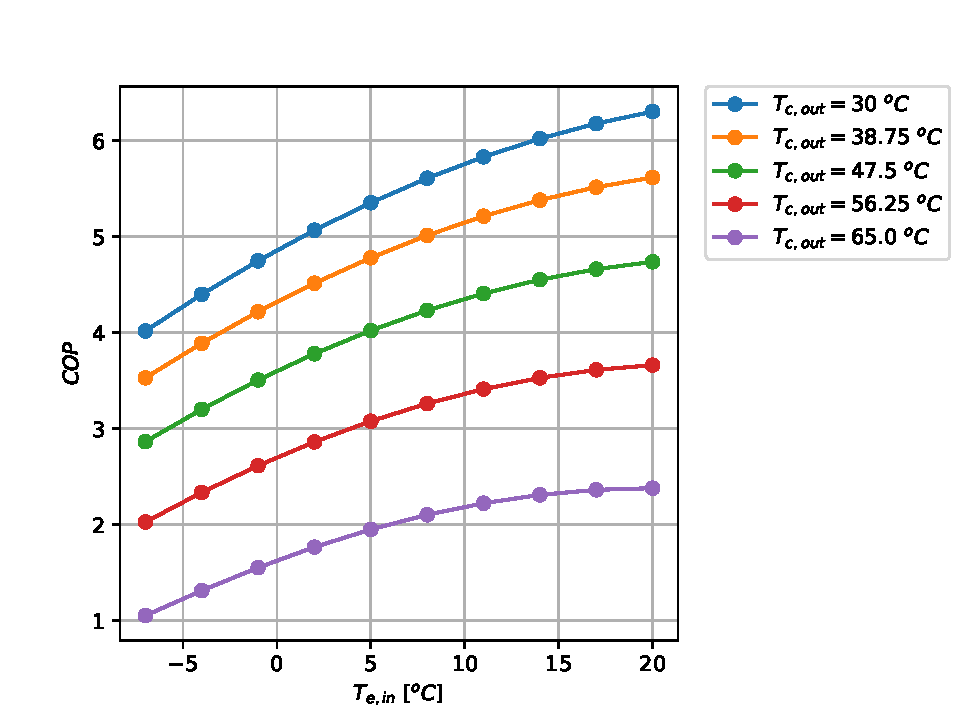
\includegraphics[width=1\textwidth]{C:/Daten/spfPackages/GIT/spfTrnsysFiles/HeatPump/BrineToWater/Walter Meier/SIN-22TU/SIN-22TU-Cop.pdf}
\caption{COP Results for the heat pump at the selected points}
\label{COPFig}
\end{center}
\end{figure}
\begin{figure}[!ht]
\begin{center}
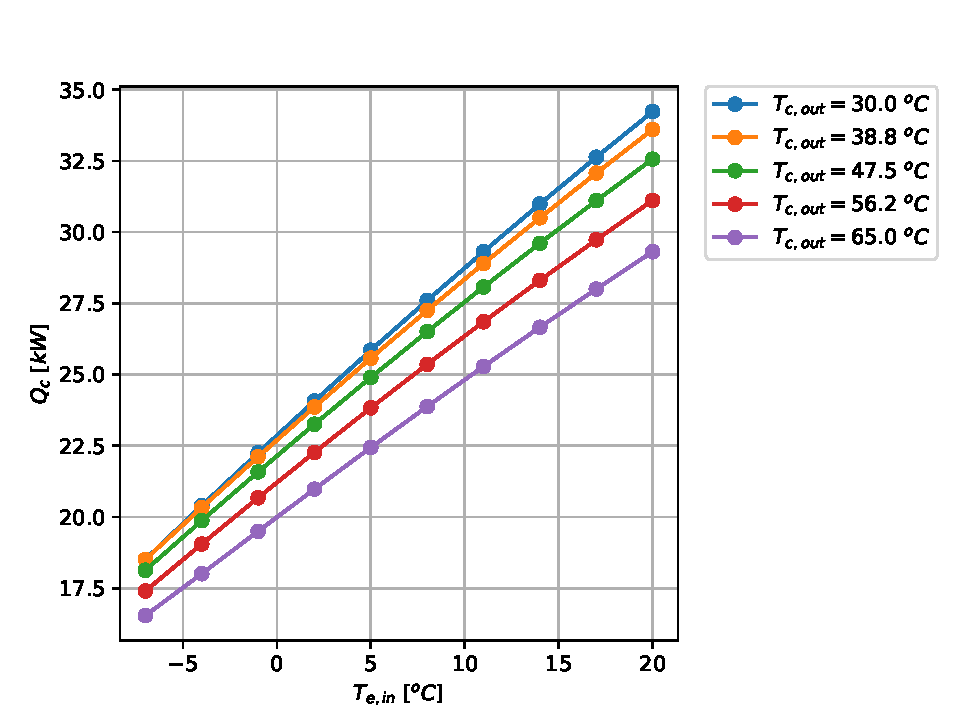
\includegraphics[width=1\textwidth]{C:/Daten/spfPackages/GIT/spfTrnsysFiles/HeatPump/BrineToWater/Walter Meier/SIN-22TU/SIN-22TU-Qc.pdf}
\caption{$Q_c$ Results for the heat pump at the selected points}
\label{QcFig}
\end{center}
\end{figure}
\end{document}
